%% -*- coding:cp1251 -*- 
\begin{figure}[h]
\centering
\begin{picture}(200,170)
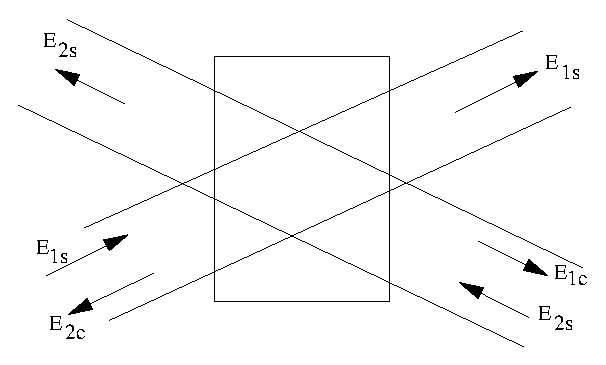
\includegraphics{./pic1.eps}
\end{picture}
\begin{picture}(200,170)(-50,0)
%middle line
\put(72,130){\line(1,1){12}}
\multiput(72,120)(0,-10){10}{\line(1,1){15}}
\put(75,120){$V$}
\put(92,125){$S$}
%E1
\put(25,20){\vector(1,1){130}}
\put(20,30){$\vec{E}_1$}
\thicklines
\put(90,85){\vector(1,1){20}}
\put(100,110){$\vec{k}_1$}
\put(90,85){\vector(1,-1){20}}
\put(95,50){$-\vec{k}_2$}
\thinlines
\qbezier (20,60) (22,65) (24,55)
\qbezier (24,55) (26,45) (28,50)
\qbezier (28,50) (32,55) (34,45)
\qbezier (34,45) (36,35) (38,40)
\qbezier (38,40) (40,45) (42,35)
\qbezier (42,35) (44,25) (46,30)
\qbezier (46,30) (50,35) (52,25)
\qbezier (52,25) (54,15) (56,20)
\qbezier (56,20) (58,25) (60,15)
%First line
\put(70,25){\line(0,1){120}}
\put(70,85){\circle*{3}}
\put(62,87){$0$}
%middle line
\put(90,25){\line(0,1){120}}
%Last line
\put(130,25){\line(0,1){120}}
\put(130,85){\circle*{3}}
\put(135,87){$d$}
%Axe
\put(45,85){\vector(1,0){110}}
\put(160,85){$z$}
\qbezier (105,85) (107,93) (100,95)
\qbezier (105,85) (107,72) (100,75)
\put(108,90){$\theta_1$}
\put(108,73){$\theta_2$}
\thicklines
\put(90,85){\vector(1,0){25}}
\put(122,75){$\vec{n}$}
\end{picture}
\end{figure}